\chapter{Resultados} \label{chap:resultados} % ### 7.

Neste capítulos serão apresentados os resultados obtidos com a \hyperref[sec:sistema]{implementação do sistema} de gerenciamento de suporte à decisão discutido ao longo deste trabalho. Serão apresentadas as \hyperref[ssec:paginas]{páginas} desenvolvidas, bem como as \hyperref[ssec:funcionalidades]{funcionalidades} implementadas.

\section{Sistema desenvolvido} \label{sec:sistema}

O sistema foi desenvolvido utilizando a linguagem de programação JavaScript em conjunto com o React, um framework de desenvolvimento de interfaces de usuário. O sistema consiste de um conjunto de \hyperref[ssec:paginas]{oito páginas} principais, das quais emergem diversas \hyperref[ssec:funcionalidades]{funcionalidades}.

\subsection{Páginas} \label{ssec:paginas}

A página inicial (\autoref{fig:pagina_main}) apresenta um resumo do objetivo e seu funcionamento básico, informa também sobre atalhos possíveis para uso mais dinâmico do sistema.
básica de dados, se mostra como uma página importante para futuros desenvolvimentos no campo de alocação de alunos em turmas.

\begin{MyCenteredFigure} \caption{Página inicial do sistema} \label{fig:pagina_main}
  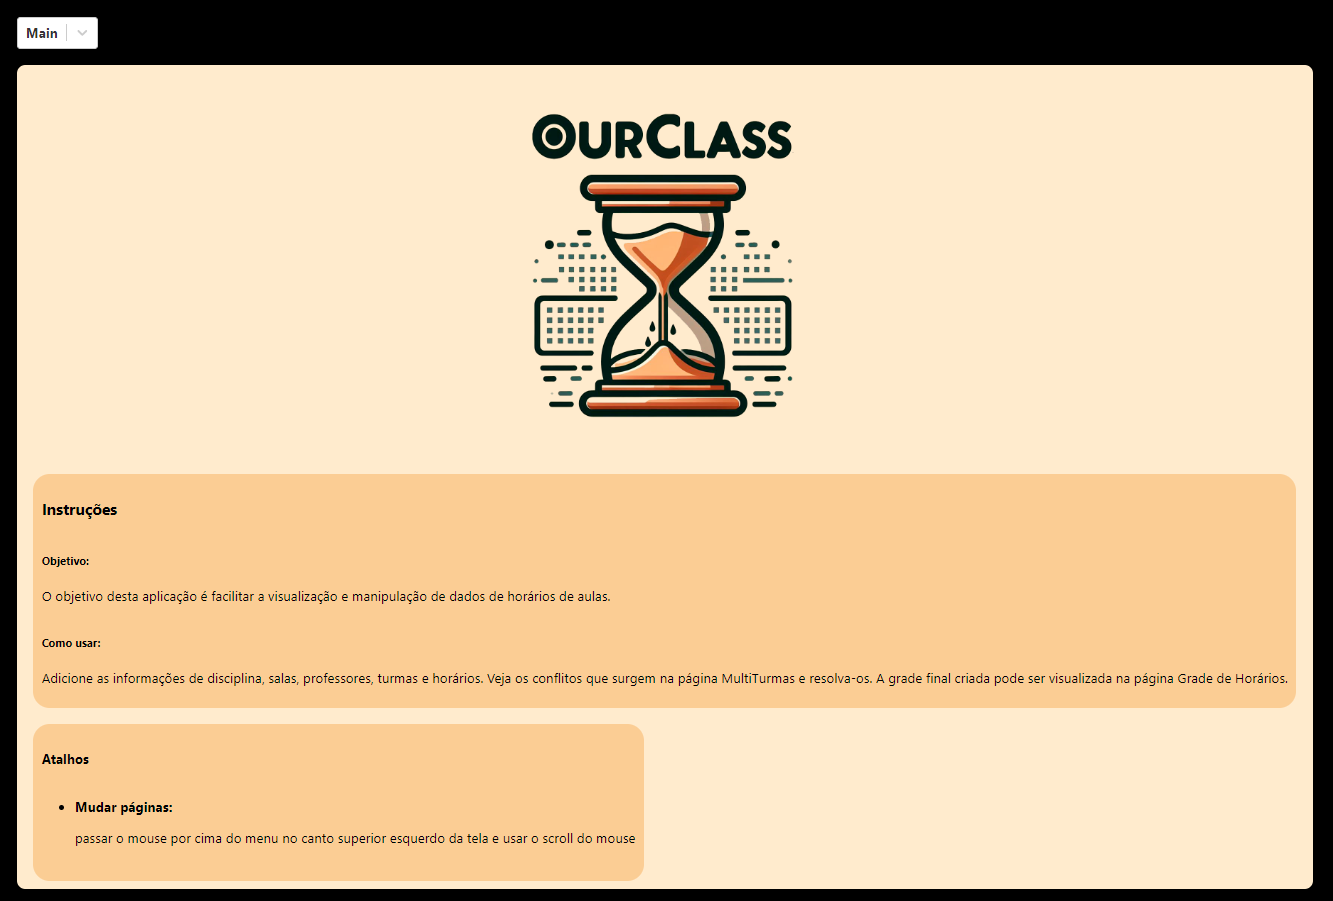
\includegraphics[width=\textwidth]{files/img/2.02!7-resultados/1-Main.png}
\end{MyCenteredFigure}

A página \textbf{MultiTurmas} é repartida em três partes principais: a primeira, com filtros para a seleção das turmas mostradas (\autoref{fig:pagina_multiFiltros}); a segunda, com a visualização dos conflitos de horários entre as turmas selecionadas (\autoref{fig:pagina_multiConflitos}); e a terceira, com a visualização das disciplinas pendentes de alocação nas turmas selecionadas (\autoref{fig:pagina_multiDisciplinas}).

\begin{MyCenteredFigure} \caption{Página de multiturmas com filtros} \label{fig:pagina_multiFiltros}
  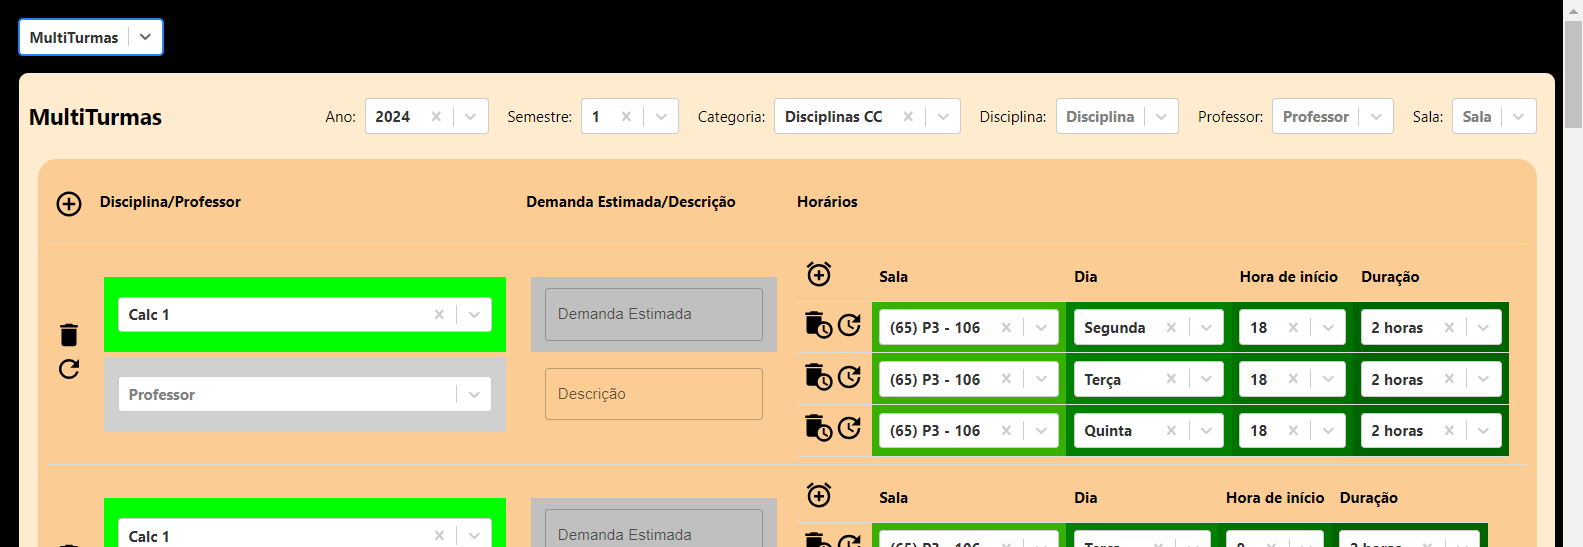
\includegraphics[width=\textwidth]{files/img/2.02!7-resultados/2-Multiturmas-Filtros.png}
\end{MyCenteredFigure}

\begin{MyCenteredFigure} \caption{Página de multiturmas com conflitos} \label{fig:pagina_multiConflitos}
  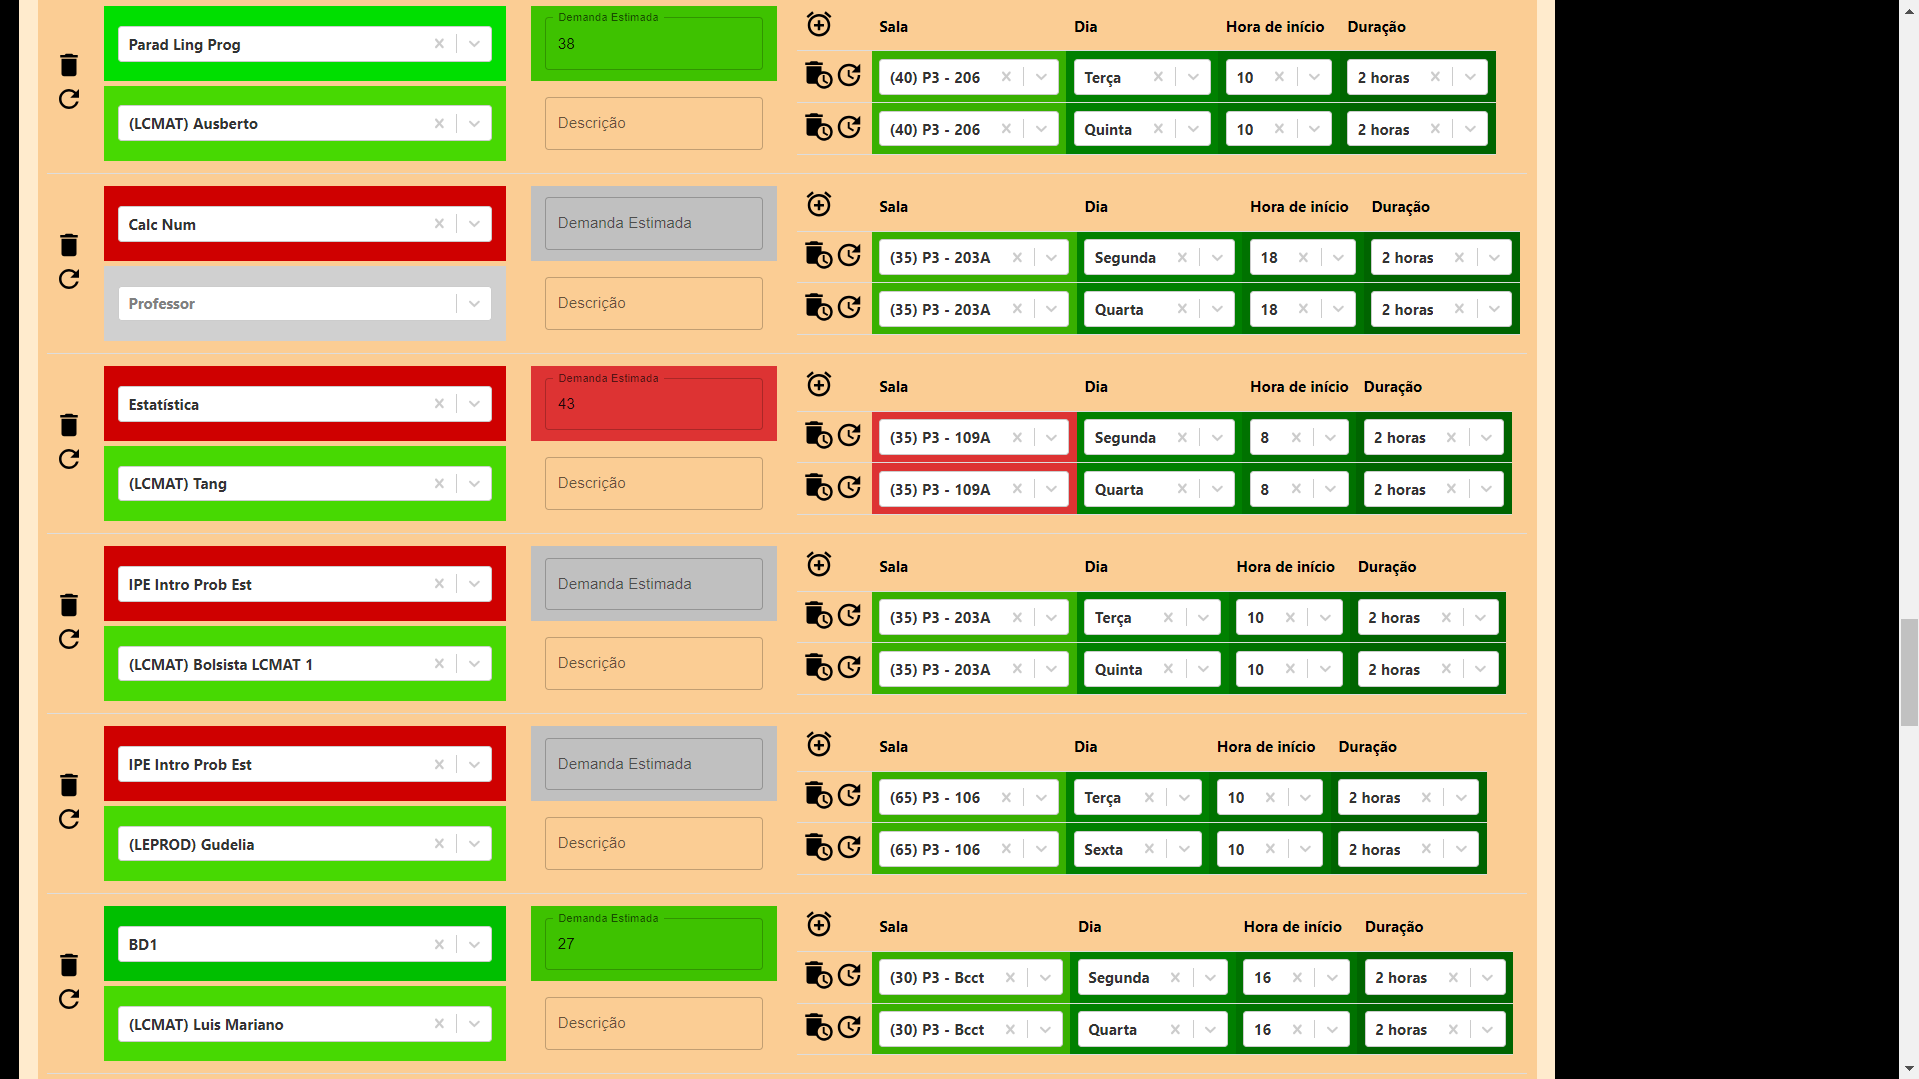
\includegraphics[width=\textwidth]{files/img/2.02!7-resultados/3-Multiturmas-Conflitos.png}
\end{MyCenteredFigure}

\begin{MyCenteredFigure} \caption{Página de multiturmas com disciplinas pendentes} \label{fig:pagina_multiDisciplinas}
  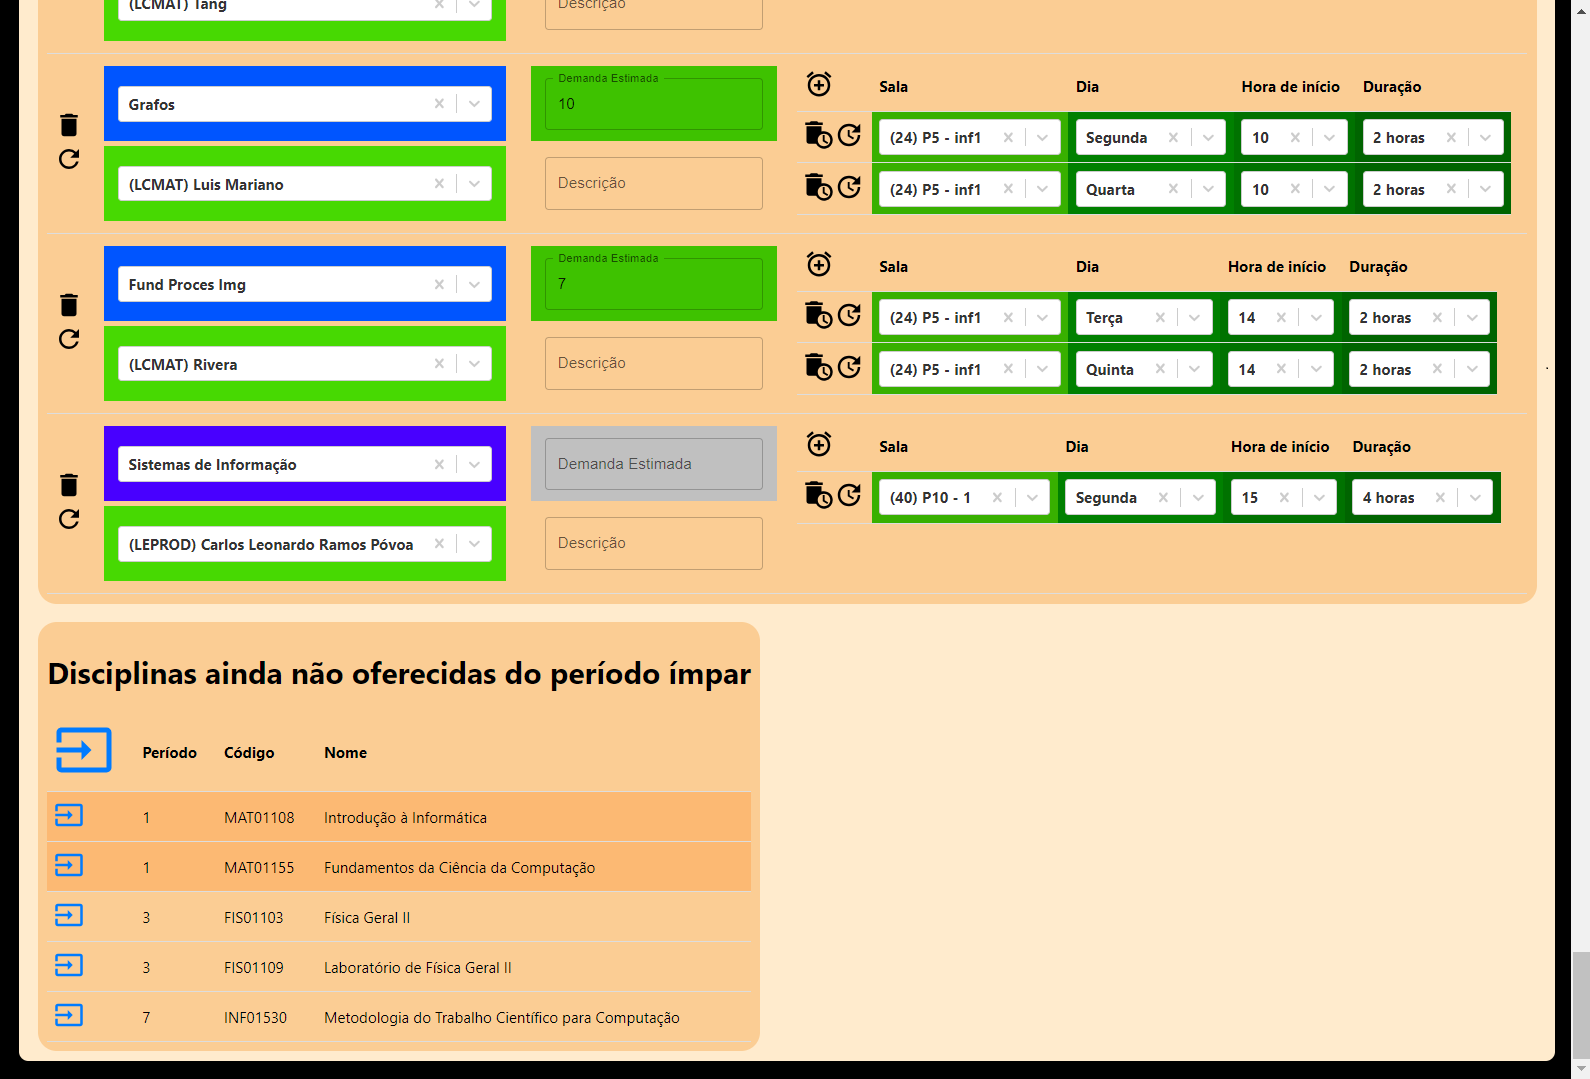
\includegraphics[width=\textwidth]{files/img/2.02!7-resultados/4-Multiturmas-DisciplinasPendentes.png}
\end{MyCenteredFigure}

A página \textbf{Grade de Horários} (\autoref{fig:pagina_grade}) apresenta a grade de horários de todas as turmas, podendo também haver a filtragem de quais turmas serão mostradas.

\begin{MyCenteredFigure} \caption{Página de grade de horários} \label{fig:pagina_grade}
  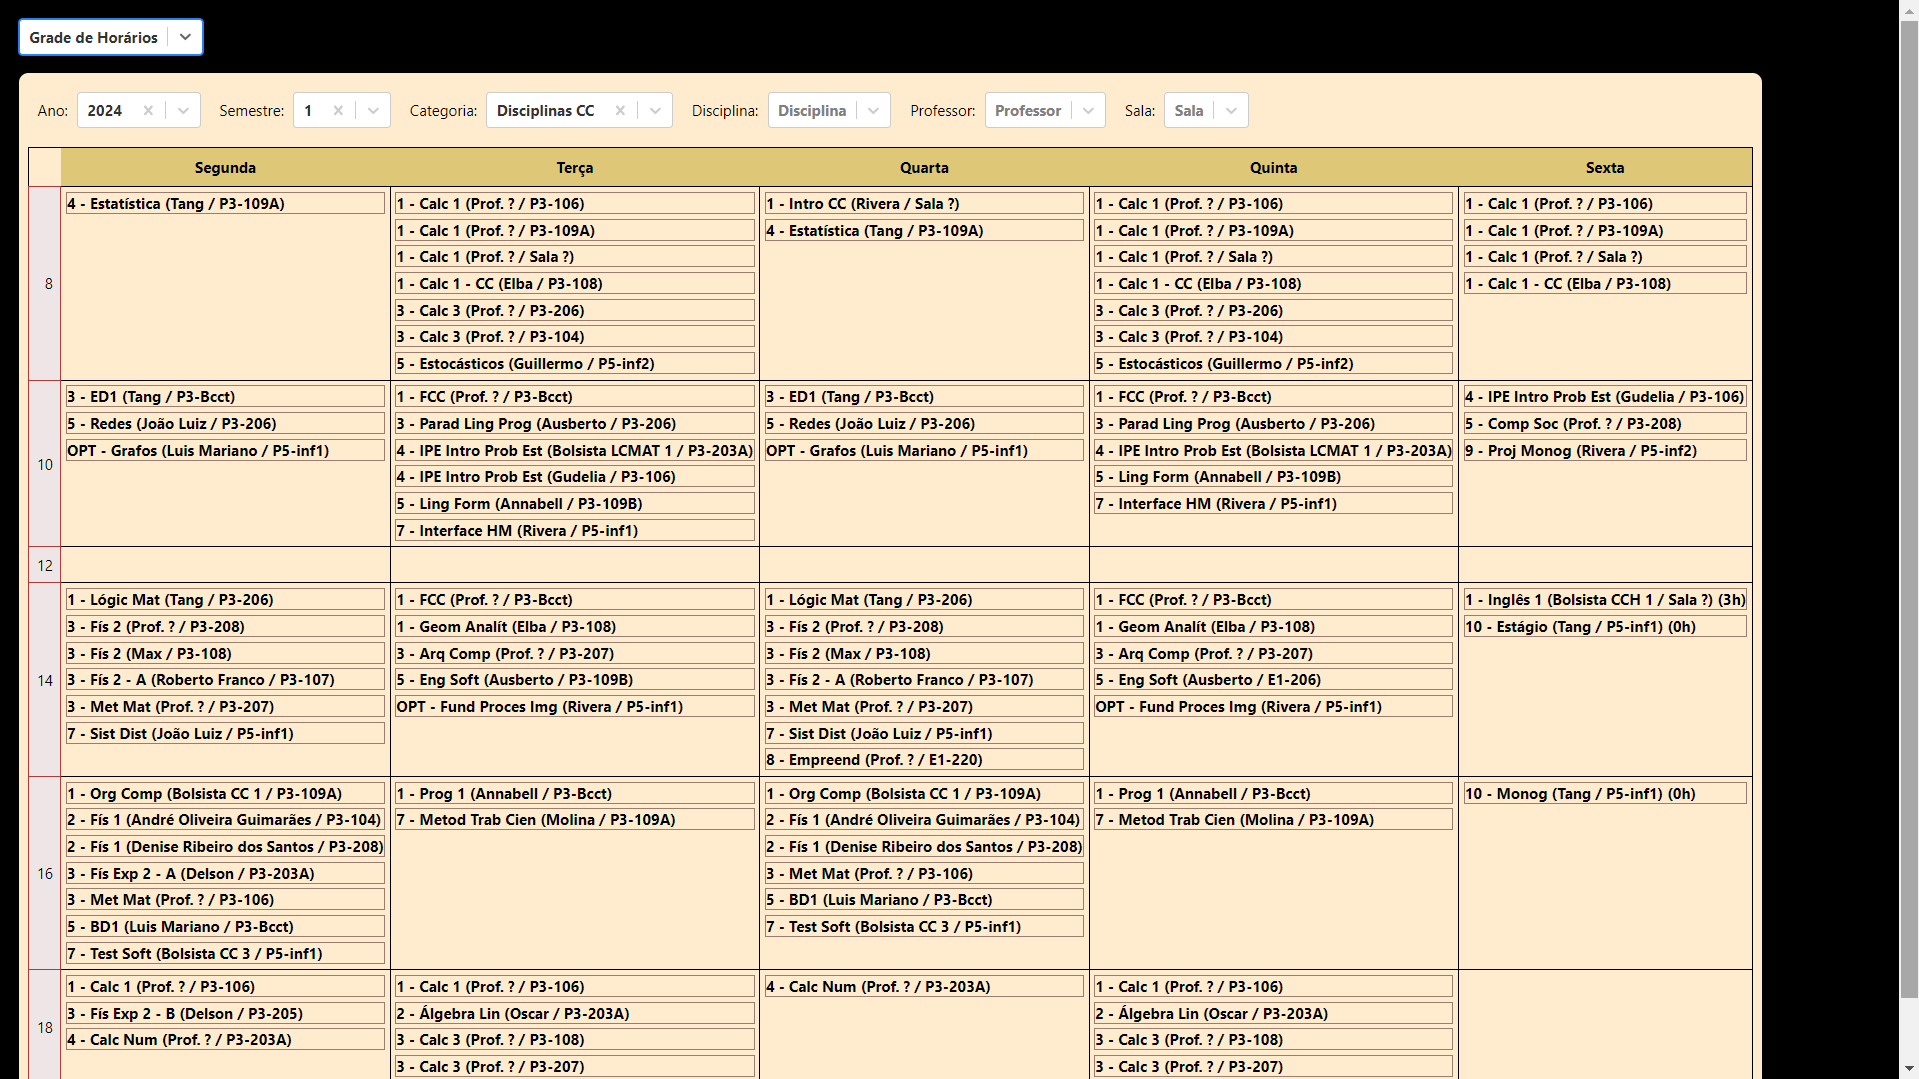
\includegraphics[width=\textwidth]{files/img/2.02!7-resultados/5-Grade de Horários.png}
\end{MyCenteredFigure}

A página \textbf{Turmas} (\autoref{fig:pagina_turmas}) apresenta todas as turmas cadastradas, podendo ser feita a edição ou exclusão individual de cada uma delas. Embora ela apresente um funcionamento similar à página MultiTurmas, tem potencial para trabalhar posteriormente com um ajuste fino específico de cada turma.

\begin{MyCenteredFigure} \caption{Página de turmas} \label{fig:pagina_turmas}
  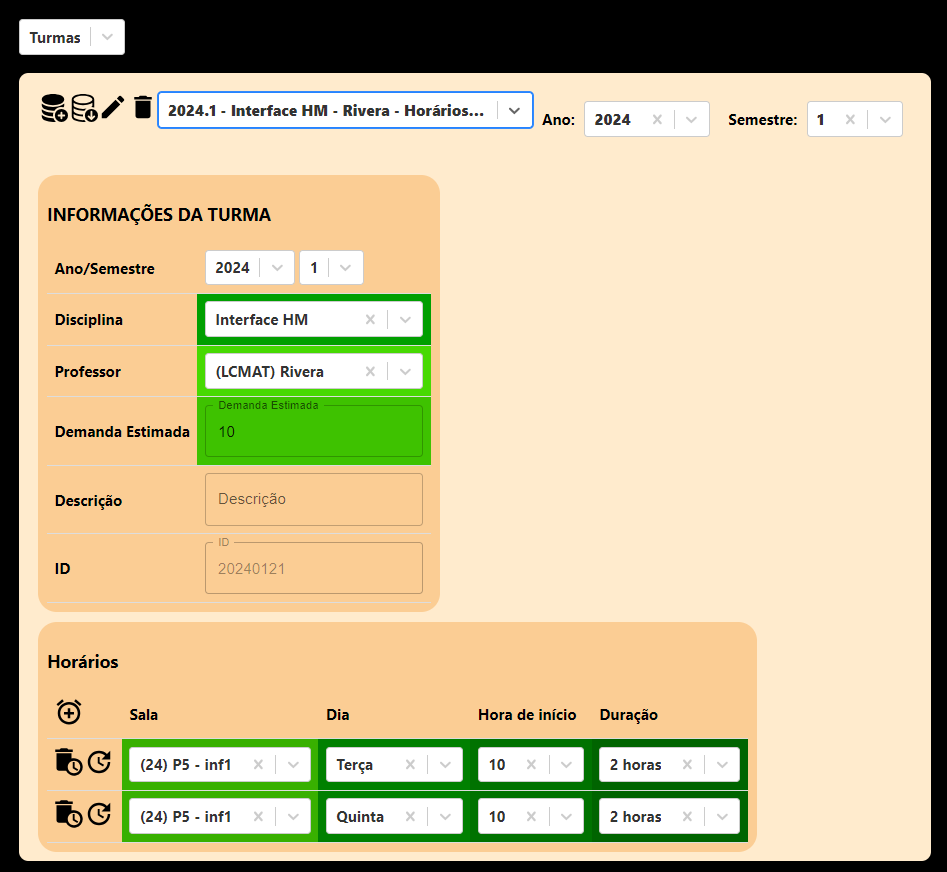
\includegraphics[width=\textwidth]{files/img/2.02!7-resultados/6-Turmas.png}
\end{MyCenteredFigure}

As páginas \textbf{Professores} (\autoref{fig:pagina_professores}), \textbf{Salas} (\autoref{fig:pagina_salas}) e \textbf{Disciplinas} (\autoref{fig:pagina_disciplinas}) apresentam um funcionamento muito similar entre si. Todas elas permitem as operações de criação, leitura, atualização e exclusão de seus respectivos itens. Além de apresentar também uma tabela inferior onde são listadas os horários histórias em que cada um desses itens foi alocado, podendo haver também a filtragem por ano, semestre, dia e hora.

\begin{MyCenteredFigure} \caption{Página de professores} \label{fig:pagina_professores}
  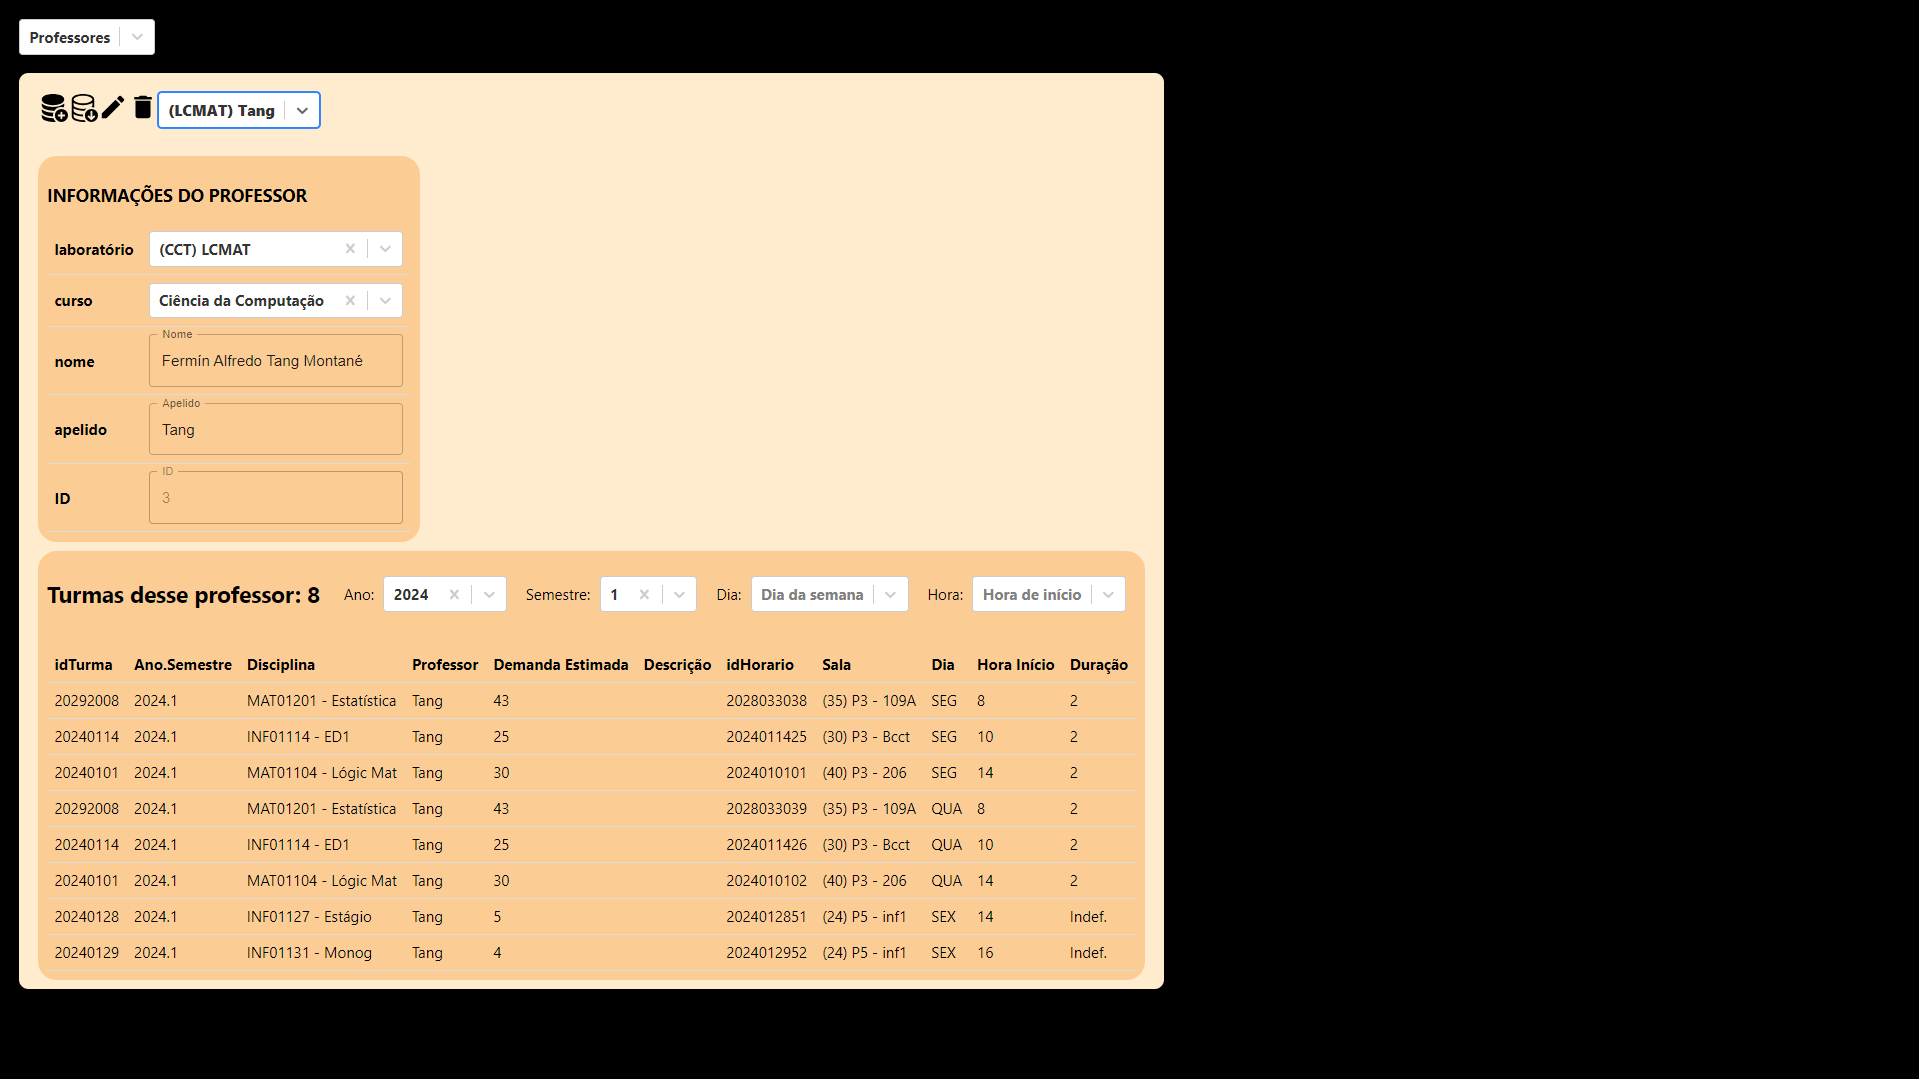
\includegraphics[width=\textwidth]{files/img/2.02!7-resultados/7-Professores.png}
\end{MyCenteredFigure}

\begin{MyCenteredFigure} \caption{Página de salas} \label{fig:pagina_salas}
  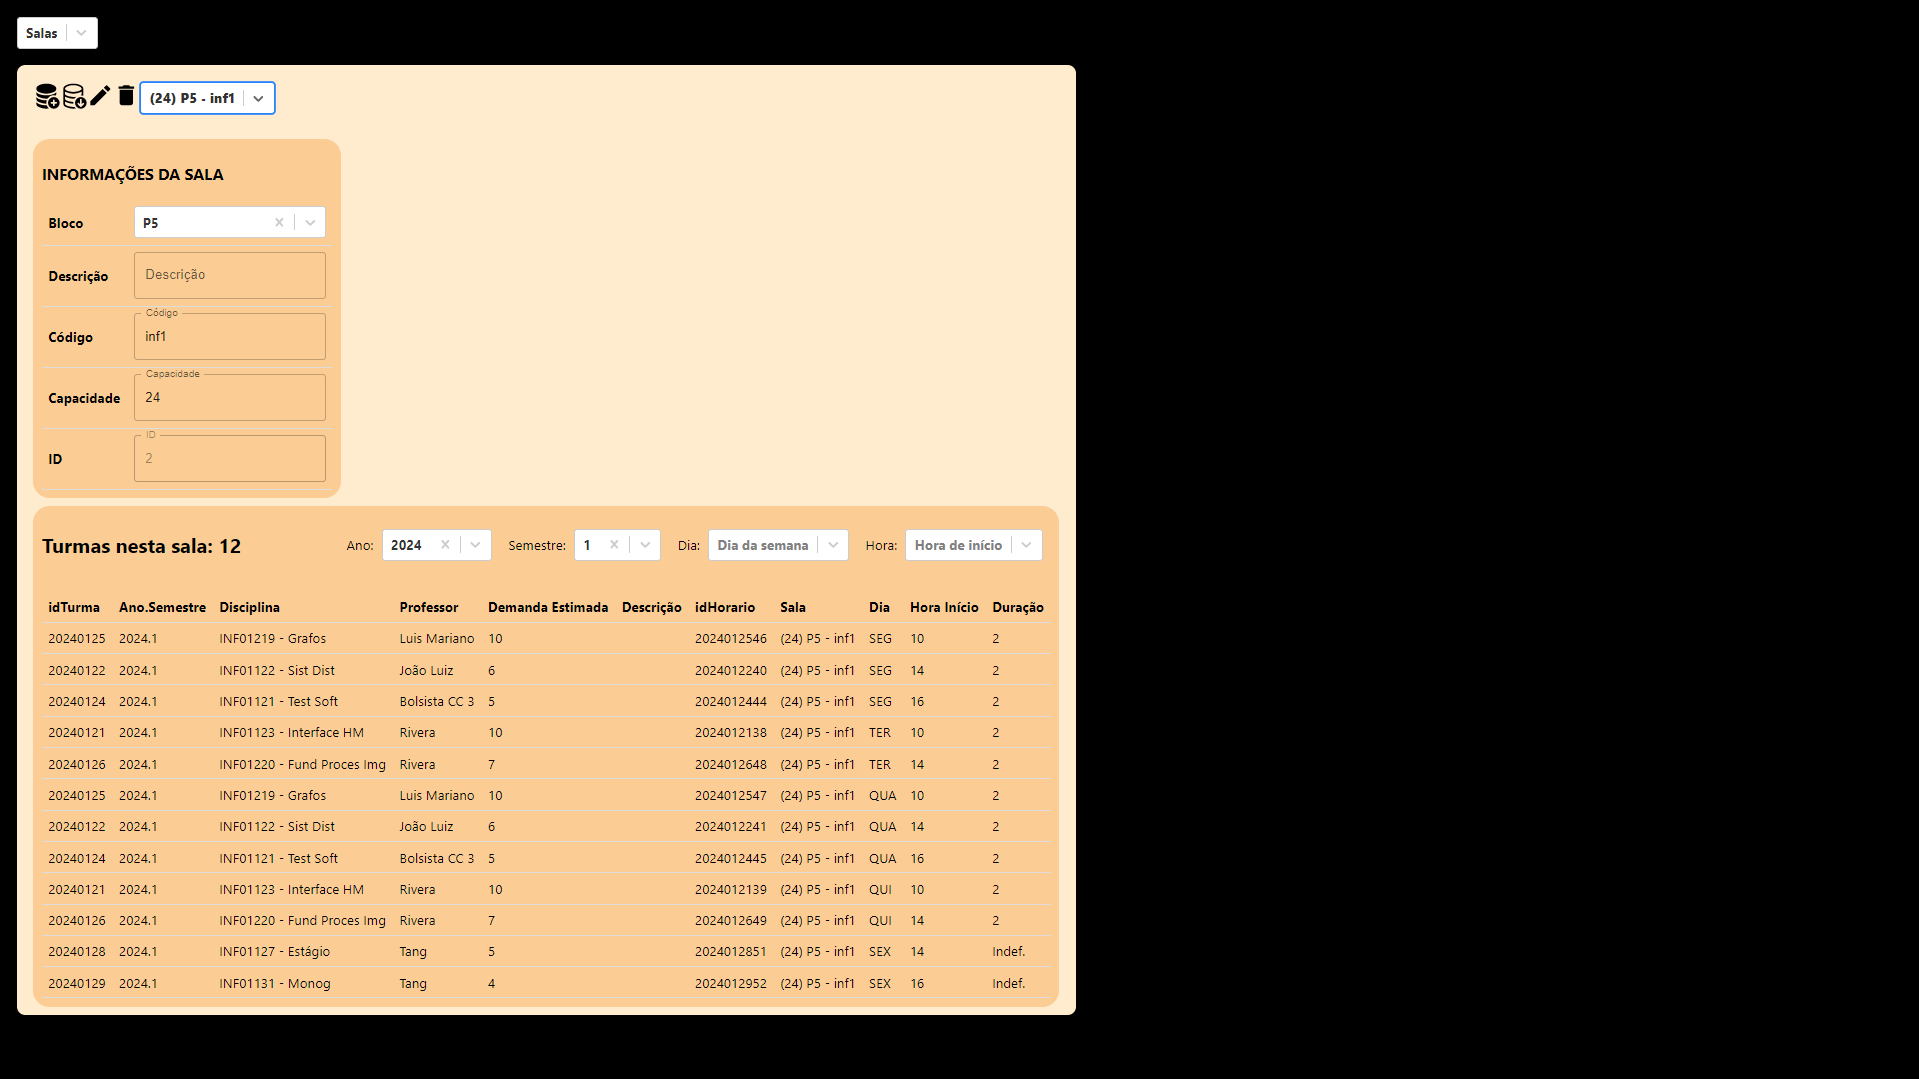
\includegraphics[width=\textwidth]{files/img/2.02!7-resultados/8-Salas.png}
\end{MyCenteredFigure}

\begin{MyCenteredFigure} \caption{Página de disciplinas} \label{fig:pagina_disciplinas}
  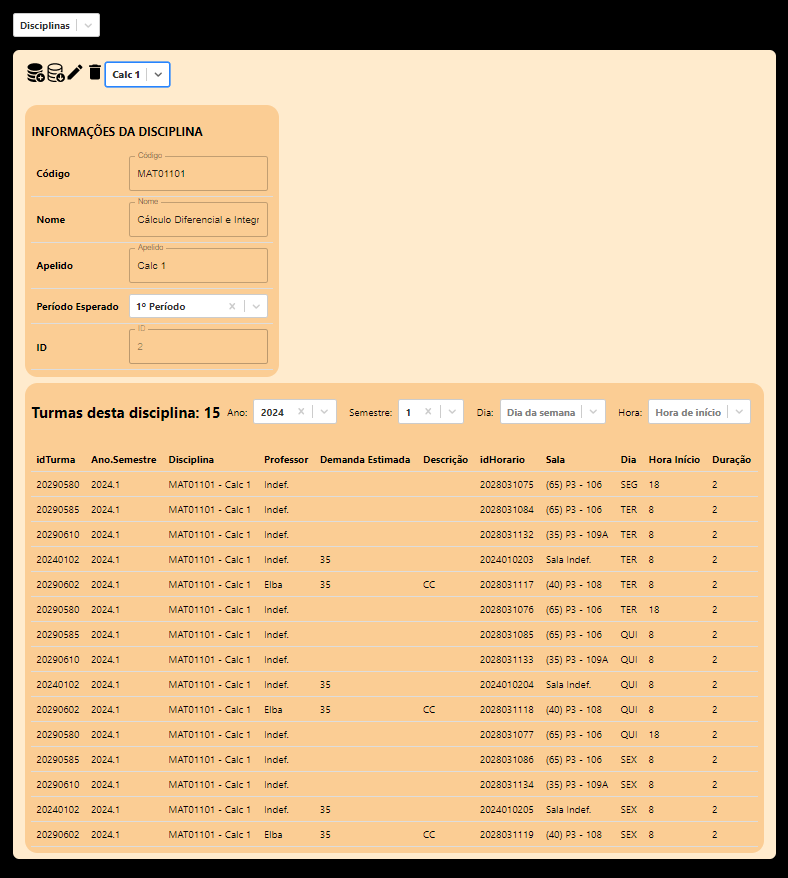
\includegraphics[width=\textwidth]{files/img/2.02!7-resultados/9-Disciplinas.png}
\end{MyCenteredFigure}

A página \textbf{Alunos} (\autoref{fig:pagina_alunos}), por fim, apresenta a possibilidade de visualização de todos os alunos cadastrados. Mesmo não possuindo funcionalidades além da manipulação

\begin{MyCenteredFigure} \caption{Página de alunos} \label{fig:pagina_alunos}
  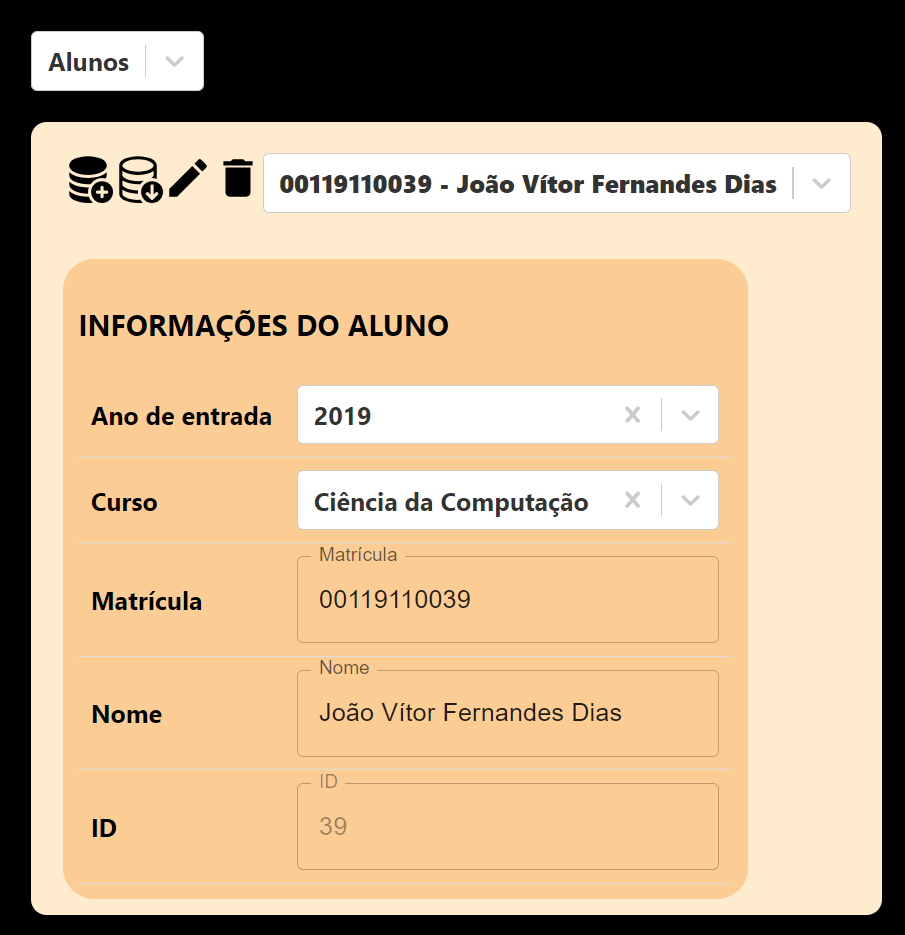
\includegraphics[width=\textwidth]{files/img/2.02!7-resultados/10-Aluno.png}
\end{MyCenteredFigure}

\subsection{Funcionalidades} \label{ssec:funcionalidades}

Nas páginas apresentadas, foram implementadas diversas funcionalidades que permitem a interação do usuário com o sistema. Dentre elas, destacam-se as \hyperref[sssec:CRUD]{quatro operações básicas de armazenamento persistente}, a \hyperref[sssec:Análise histórica]{análise histórica}, a \hyperref[sssec:Criação de grade inicial]{criação de grade inicial}, a \hyperref[sssec:Visualização de conflitos]{Visualização de conflitos} e a \hyperref[sssec:Visualização de tabelas horárias]{visualização das tabelas horárias}.

\subsubsection*{CRUD} \label{sssec:CRUD}

Com exceção da página inicial e da página de grade de horários, todas as páginas apresentam as operações de criação, leitura, atualização e exclusão de seus respectivos itens. Isso se dá pois esta é a função básica de um sistema de gerenciamento de banco de dados, sendo necessária para que todas as outras funcionalidades possam ser implementadas e utilizáveis.

\subsubsection*{Análise histórica} \label{sssec:Análise histórica}

O conceito da \textbf{Análise Histórica} é a capacidade de visualizar quais foram todos os horários em que um determinado item foi alocado. Isso é útil para avaliar os padrões emergentes nas alocações dos recursos.

\subsubsection*{Criação de grade inicial} \label{sssec:Criação de grade inicial}

A \textbf{Criação de Grade Inicial}, já descritas no \hyperref[ssec:Heurística]{segmento sobre heurística de criação de grade}, é uma funcionalidade que permite a criação de uma grade de horários inicial através da avaliação das alocações anteriores para determinada disciplina. Através dela é possível criar uma grade de horários inicial para o curso de Ciência da Computação em poucos segundos.

\subsubsection*{Visualização de conflitos} \label{sssec:Visualização de conflitos}

Na página \textbf{Turmas} e principalmente na página \textbf{MultiTurmas}, é possível visualizar os conflitos existentes entre as turmas. Os \hyperref[sec:conflitos]{conflitos} são apresentados de forma clara e objetiva, permitindo a rápida identificação e posterior resolução.

\subsubsection*{Visualização de tabelas horárias} \label{sssec:Visualização de tabelas horárias}

Por fim, especificamente na página \textbf{Grade de Horários}, é possível visualizar as tabelas horárias de todas as turmas cadastradas, podendo haver também a filtragem por ano, semestre, categoria, disciplina, professor e sala. Com esta visualização tabular, pode-se gerar as grades de horários específicas das turmas de disciplinas de cada um dos períodos letivos, bem como distingue as turmas entre as que pertencem à ementa do Curso de Ciência da Computação e as que não pertencem.

Assim como no caso da \hyperref[sssec:Análise histórica]{análise histórica}, a visualização das tabelas horárias é uma funcionalidade que permite a visualização de padrões emergentes nas alocações dos recursos.

\section{Ferramentas disponíveis para gestão dos horários} % ### 7.2.

Além do desenvolvimento para auxílio na criação da grade horária, ao longo do estudo, o presente trabalho também encontrou métodos alternativos para se amenizar a problemática abordada. Sendo, de forma simples, o uso de ferramentas burocráticas disponíveis na instituição que abrem alguns caminhos para uma maior maleabilidade no processo de resolução do problema. Entretanto, é necessário que se tenha em mente que a burocracia é um processo lento e que pode ser desgastante, sendo até mesmo esperado que não seja desejado por parte dos construtores da grade horária.

Essas alternativas não geram por si só uma solução para o problema, mas servem como meios possíveis para se realizar mudanças além das usuais.

\subsection{Tempo de elaboração das grades} \label{ssec:burocracia-férias} % #### 7.1.1.

Durante as entrevistas do \autoref{chap:instituicao} da \autoref{sec:entrevistas}, uma alternativa válida para a amenização da problemática abordada é a alteração do calendário anual da UENF que define férias de duas semanas entre os semestres. Caso seu calendário seja alterado para que as férias sejam de três semanas, o problema de agendamento teria maior tempo para ser resolvido, assim fazendo com que a solução ótima seja provável de ser alcançada.

% Citar o Estatuto da forma correta.

Segundo o Artigo 28 do Estatuto da UENF \cite{Estatuto2002}, compete à secretaria acadêmica a elaboração da proposta de calendário escolar para que seja aprovado pelo Colegiado Acadêmico. Enquanto que o Artigo 63 da seção 2 do capítulo 1, informa que os calendários do curso de graduação devem ser aprovados pelas correspondentes câmaras, com observância do calendário da universidade.

Logo, quanto à alteração do calendário acadêmico, a alteração mostra-se como possível, sendo necessário apenas que o processo burocrático necessário seja enfrentado, o que pode acabar não sendo do desejo daqueles que constroem a grade horária.

\subsection{Alteração forçada de horários} \label{ssec:burocracia-troca} % #### 7.1.2.

Segundo o parágrafo primeiro do artigo 36 das Normas de Graduação \cite{Normas2012}, ``qualquer alteração de horário/turno após o período de matrícula deverá ter a anuência por escrito de todos os discentes matriculados na turma''. Seguindo ao segundo parágrafo do mesmo artigo, temos que ``a alteração de horário das aulas da turma deverá ter a anuência da Coordenação de Curso e a ciência do Chefe do Laboratório responsável pela disciplina''.

Outra alternativa que aproveita de uma brecha nas normas supracitadas é a possibilidade de se criar novas turmas para as disciplinas que possuem horários conflitantes, assim direcionando os alunos para que se desinscrevam da turma anterior.

Ambas as alternativas supracitadas visam a alteração dos horários das turmas mesmo após o estimado período de construção da grade horária, assim efetivamente aumentando novamente o tempo disponível para a resolução do problema.

% Art. 36 As aulas deverão ser ministradas pelo Docente responsável da disciplina
% nos horários designados pela Coordenação de Curso.
% 13
% § 1º Qualquer alteração de horário/turno após o período de matrícula deverá
% ter a anuência por escrito de todos os discentes matriculados na turma.
% § 2º º A alteração de horário das aulas da turma deverá ter a anuência da
% Coordenação de Curso e a ciência do Chefe do Laboratório responsável pela
% disciplina.

\subsection{Aplicação prática dos métodos burocráticos} \label{ssec:aplicacaoDasMudancas} % #### 7.1.3.

% O QUE DEVERIA TER INTERVALO É ENTRE O FIM DAS INSCRIÇÕES E O INÍCIO DAS AULAS

% adicionar também a possibilidade da mudança informal do horário

Consideremos o ano de 2023, os seus semestres e seus respectivos calendário acadêmicos \cite{Calendario2023_1,Calendario2023_2} para a graduação, onde a \autoref{tab:calendario_SECACAD-2023.1} mostra o calendário do primeiro semestre e a \autoref{tab:calendario_SECACAD-2023.2} mostra o calendário do segundo semestre.

% Abreviados
\begin{table}[H] \centering \caption{Calendário Acadêmico da SECACAD de 2023.1 (simplificado)} \label{tab:calendario_SECACAD-2023.1}
  \begin{tabular}{| l r |}
    \hline
    \textbf{Atividades}                                              & \textbf{Data} \\
    \hline
    Prazo limite de cad. de nov. discip. a serem ofer. em 2023.1     & até 20/01     \\
    Prazo limite para criação de turmas a serem oferecidas em 2023.1 & 20/01 a 15/02 \\
    Renovação de matrícula de 2023.1                                 & 28/02 a 03/03 \\
    Início do período letivo de 2023.1                               & 06/03         \\
    Inclusão e exclusão de disciplinas                               & 06/03 à 20/03 \\
    Encerramento do período letivo de 2023.1                         & 07/07         \\
    Prazo limite: Entrega dos resultados à SECACAD                   & 14/07         \\
    \hline
  \end{tabular}
\end{table}

% as is
\begin{comment}
\begin{table}[H] \centering
  \caption{Calendário Acadêmico da SECACAD de 2023.1 (simplificado)}
  \label{tab:calendario_SECACAD-2023.1}
  \begin{tabular}{| l r |}
    \hline
    \textbf{Atividades}                                                                           & \textbf{Data}           \\
    \hline
    Prazo limite de cadastro de novas disciplinas a serem oferecidas no 1º período letivo de 2023 & até 20/01/2023          \\
    Prazo limite para criação de turmas a serem oferecidas no 1º período letivo de 2023           & 20/01/2023 a 15/02/2023 \\
    Renovação de matrícula do 1º período letivo/2023                                              & 28/02 a 03/03           \\
    Início do 1º período letivo de 2023                                                           & 06/03                   \\
    Inclusão e exclusão de disciplinas                                                            & 06/03 à 20/03           \\
    Encerramento do 1º período letivo de 2023                                                     & 07/07                   \\
    \hline
  \end{tabular}
\end{table}

\begin{table}[H] \centering
  \caption{Calendário Acadêmico da SECACAD de 2023.2 (simplificado)}
  \label{tab:calendario_SECACAD-2023.2}
  \begin{tabular}{| l r |}
    \hline
    \textbf{Atividades}                                                                           & \textbf{Data} \\
    \hline
    Prazo limite de cadastro de novas disciplinas a serem oferecidas no 2º período letivo de 2023 & até 14/07     \\
    Prazo limite: Entrega dos resultados à SECACAD                                                & 14/07         \\
    Prazo limite para criação de turmas a serem oferecidas no 2º período letivo de 2023           & 17 a 28/07    \\
    Renovação de matrícula do 2º período letivo/2023                                              & 01/08 a 04/08 \\
    Início do 2º período letivo de 2023                                                           & 07/08         \\
    Inclusão e exclusão de disciplinas                                                            & 14 a 21/08    \\
    Encerramento do 2º período letivo de 2023                                                     & 08/12         \\
    Prazo limite: Entrega dos resultados à SECACAD                                                & 15/12         \\
    \hline
  \end{tabular}
\end{table}
\end{comment}

\begin{table}[H] \centering \caption{Calendário Acadêmico da SECACAD de 2023.2 (simplificado)} \label{tab:calendario_SECACAD-2023.2}
  \begin{tabular}{| l r |}
    \hline
    \textbf{Atividades}                                              & \textbf{Data} \\
    \hline
    Prazo limite de cad. de nov. discip. a serem ofer. em 2023.2     & até 14/07     \\
    Prazo limite para criação de turmas a serem oferecidas em 2023.2 & 17 a 28/07    \\
    Renovação de matrícula de 2023.2                                 & 01/08 a 04/08 \\
    Início do período letivo de 2023.2                               & 07/08         \\
    Inclusão e exclusão de disciplinas                               & 14 a 21/08    \\
    Encerramento do período letivo de 2023.2                         & 08/12         \\
    Prazo limite: Entrega dos resultados à SECACAD                   & 15/12         \\
    \hline
  \end{tabular}
\end{table}

Com objetivo de tormar a visualização das informações mais coesa, a \autoref{tab:calendario_2023-Enxuto} mostra um calendário acadêmico normalizado, onde os prazos, períodos e marcações de início e fim foram convertidos em termos de ``início'' e ``fim'', assim distinguindo também o seu período de vigência e a data específica.

\begin{table}[H] \centering \caption{Calendário Acadêmico de 2023 (simplificado)} \label{tab:calendario_2023-Enxuto}
  \begin{tabular}{| c r l c |}
    \hline
    \textbf{Vigência} & \textbf{Fase}         & \textbf{Atividades}                              & \textbf{Data} \\
    \hline
    % 2022.2          & \textbf{Fim}          & período letivo                                   & 14/12/22      \\
    % 2022.2          & \textbf{\textit{Fim}} & entrega dos resultados à SECACAD                 & 21/12/22      \\

    2023.1            & \textbf{\textit{Fim}} & cadastro de novas disciplinas a serem oferecidas & 20/01/23      \\
    2023.1            & \textbf{Início}       & criação de turmas a serem oferecidas             & 20/01/23      \\
    2023.1            & \textbf{Fim}          & criação de turmas a serem oferecidas             & 15/02/23      \\
    2023.1            & \textbf{Início}       & renovação de matrícula                           & 28/02/23      \\
    2023.1            & \textbf{Fim}          & renovação de matrícula                           & 03/03/23      \\
    2023.1            & \textbf{Início}       & período letivo                                   & 06/03/23      \\
    2023.1            & \textbf{Início}       & inclusão e exclusão de disciplinas               & 06/03/23      \\
    2023.1            & \textbf{Fim}          & inclusão e exclusão de disciplinas               & 20/03/23      \\
    2023.1            & \textbf{Fim}          & período letivo                                   & 07/07/23      \\
    2023.1            & \textbf{\textit{Fim}} & entrega dos resultados à SECACAD                 & 14/07/23      \\

    2023.2            & \textbf{\textit{Fim}} & cadastro de novas disciplinas a serem oferecidas & 14/07/23      \\
    2023.2            & \textbf{Início}       & criação de turmas a serem oferecidas             & 17/07/23      \\
    2023.2            & \textbf{Fim}          & criação de turmas a serem oferecidas             & 28/07/23      \\
    2023.2            & \textbf{Início}       & renovação de matrícula                           & 01/08/23      \\
    2023.2            & \textbf{Fim}          & renovação de matrícula                           & 04/08/23      \\
    2023.2            & \textbf{Início}       & período letivo                                   & 07/08/23      \\
    2023.2            & \textbf{Início}       & inclusão e exclusão de disciplinas               & 14/08/23      \\
    2023.2            & \textbf{Fim}          & inclusão e exclusão de disciplinas               & 21/08/23      \\
    2023.2            & \textbf{Fim}          & período letivo                                   & 08/12/23      \\
    2023.2            & \textbf{\textit{Fim}} & entrega dos resultados à SECACAD                 & 15/12/23      \\

    % 2024.1          & \textbf{Início}       & renovação de matrícula                           & 26/02/24      \\
    % 2024.1          & \textbf{Fim}          & renovação de matrícula                           & 01/03/24      \\
    % 2024.1          & \textbf{Início}       & período letivo                                   & 04/03/24      \\
    \hline
  \end{tabular}
\end{table}

Levando em consideração as ações sugeridas na \autoref{ssec:burocracia-férias} e na \autoref{ssec:burocracia-troca}, um cronograma alterado seria o disposto na \autoref{tab:calendario_2023-Alterado}, onde as ações sugeridas foram aplicadas. Essas ações incluem a alteração do calendário acadêmico para que todo o primeiro semestre comece suas atividades uma semana antes. Além disso, define-se que o período final de criação de turmas não é efetivamente finalizado no antes da renovação de matrícula, mas sim após a finalização da inclusão e exclusão de disciplinas.

Nota-se que o único caso em que não foi feita a migração exata de uma semana foi na renovação de matrícula, visto que caso fosse alterada para uma semana exata, a renovação de matrícula seria feita no período de carnaval, o que não é desejado. Assim, foi mantido o mesmo intervalo de tempo, porém, começando após o feriado nacional ``Quarta-feira de Cinzas''.

\begin{table}[H] \centering \caption{Calendário Acadêmico de 2023 - Alterado} \label{tab:calendario_2023-Alterado}
  \begin{tabular}{| c r l r |}
    \hline
    \textbf{Vigência} & \textbf{Fase}         & \textbf{Atividades}                & \textbf{Data}                  \\
    \hline
    2023.1            & \textbf{\textit{Fim}} & cadastro de novas disciplinas      & \sout{20/01} 13/01/23 \altered \\
    2023.1            & \textbf{Início}       & criação de turmas                  & \sout{20/01} 13/01/23 \altered \\ \removeLine
    \sout{2023.1}     & \sout{\textbf{Fim}}   & \sout{criação de turmas}           & \sout{15/02/23}                \\
    2023.1            & \textbf{Início}       & renovação de matrícula             & \sout{28/02} 23/02/23 \altered \\
    2023.1            & \textbf{Fim}          & renovação de matrícula             & \sout{03/03} 26/02/23 \altered \\
    2023.1            & \textbf{Início}       & período letivo                     & \sout{06/03} 27/02/23 \altered \\
    2023.1            & \textbf{Início}       & inclusão e exclusão de disciplinas & \sout{06/03} 27/02/23 \altered \\
    2023.1            & \textbf{Fim}          & inclusão e exclusão de disciplinas & \sout{20/03} 13/03/23 \altered \\ \addLine
    2023.1            & \textbf{Fim}          & criação de turmas                  & 20/03/23                       \\
    2023.1            & \textbf{Fim}          & período letivo                     & \sout{07/07} 30/06/23 \altered \\
    2023.1            & \textbf{\textit{Fim}} & entrega dos resultados à SECACAD   & \sout{14/07} 07/07/23 \altered \\

    2023.2            & \textbf{\textit{Fim}} & cadastro de novas disciplinas      & 14/07/23                       \\
    2023.2            & \textbf{Início}       & criação de turmas                  & 17/07/23                       \\ \removeLine
    \sout{2023.2}     & \sout{\textbf{Fim}}   & \sout{criação de turmas}           & \sout{28/07/23}                \\
    2023.2            & \textbf{Início}       & renovação de matrícula             & 01/08/23                       \\
    2023.2            & \textbf{Fim}          & renovação de matrícula             & 04/08/23                       \\
    2023.2            & \textbf{Início}       & período letivo                     & 07/08/23                       \\
    2023.2            & \textbf{Início}       & inclusão e exclusão de disciplinas & 14/08/23                       \\
    2023.2            & \textbf{Fim}          & inclusão e exclusão de disciplinas & 21/08/23                       \\ \addLine
    2023.2            & \textbf{Fim}          & criação de turmas                  & 21/08/23                       \\
    2023.2            & \textbf{Fim}          & período letivo                     & 08/12/23                       \\
    2023.2            & \textbf{\textit{Fim}} & entrega dos resultados à SECACAD   & 15/12/23                       \\
    \hline
  \end{tabular}
\end{table}

Com a utilização desses dois métodos burocráticos, aqueles encarregados de realizar a criação e alocação das turmas nos devido horários disporá de uma semana extra no segmento entre os semestres, assim abrindo uma janela de tempo maior para a manipulação dos horários, e consequentemente, ampliando possibilidade de se alcançar uma solução ótima.
